%!TEX root = main_ISMB.tex
\section{Supplementary data}
\subsection{Benchmark \ourprog vs \RNAinverse}
Using the same dataset of $50$ structures, we generated $100$ samples
per structure with \RNAinverse. They yield for most parameters
a high entropy. We present for every different concentration of \texttt{C+G}
the average sample entropy and the average base pairs entropy.


\begin{figure}[ht!]
	%\centering
	\hspace{-5em}
	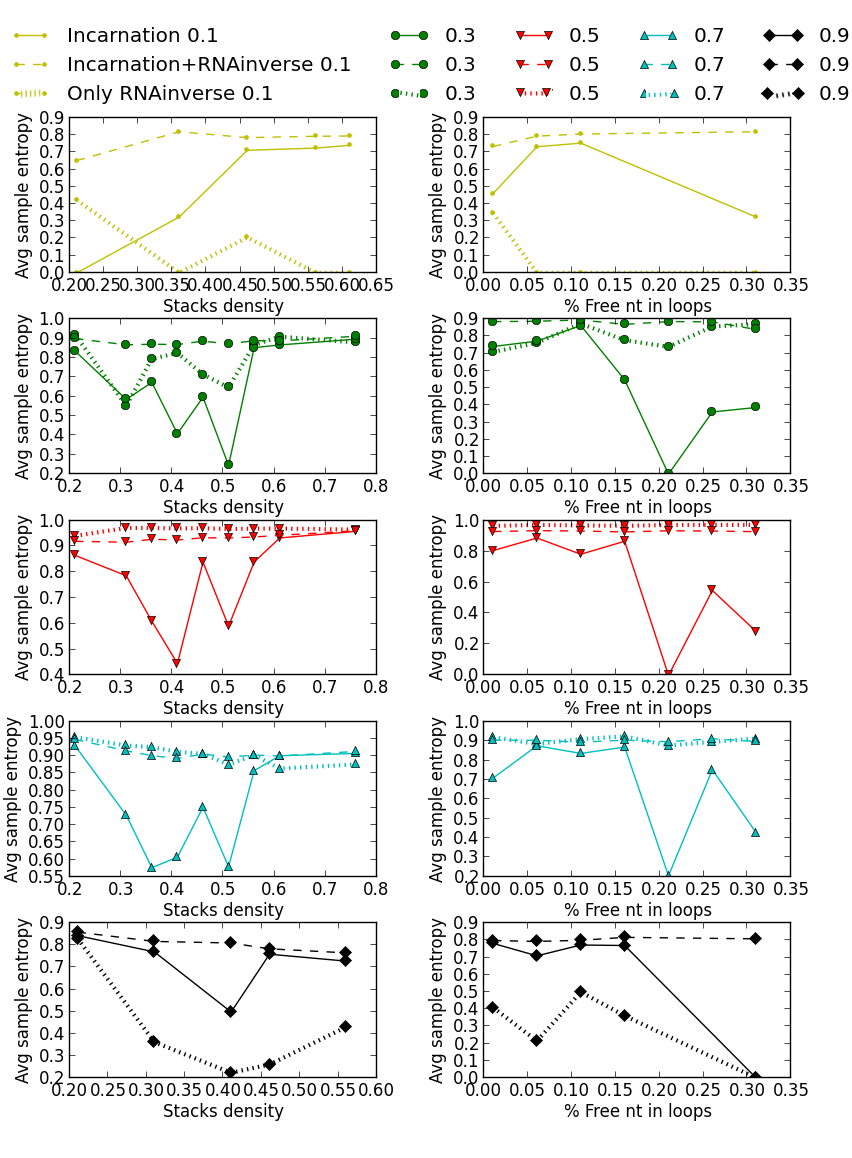
\includegraphics[scale=0.4]{Figures/RNAinverse_data_100.png}
	\caption{Entropy and \texttt{C+G} content.}
	\label{fig:rnainverse}
\end{figure}

\subsection{Impact of local search on the \gc~content of \ourprog output}

These data demonstrate that the local search heuristic used to design nucleotides in loop regions has a very limited impact on the \gc content. For each class of \gc~content, we show in Table~\ref{table:impact_on_gc}, the observed \gc~content of the sequence sampled by \ourprog, and then we report the observed \gc~content after the \RNAinverse step (as defined in Section \ref{subsec:glocal_method}). Our results show that the \gc~content is relatively well conserved. 

\begin{table}[h!]
\begin{center}
\begin{tabular}{|c|c|c|}
\hline
target \gc & \ourprog & \ourprog + \RNAinverse \\
\hline
10 & 0.15 & 0.21\\
30 & 0.30 & 0.33\\
50 & 0.48 & 0.49\\
70 & 0.71 & 0.69\\
90 & 0.83 & 0.78\\
\hline
\end{tabular}
\end{center}
\caption{Observed \gc~content of solutions returned by \ourprog (2nd column) and after the application of the local search heuristic (3rd column).}
\label{table:impact_on_gc}
\end{table}